\chapter{Design ESB in Openshift}
\label{cha:esboc}
As discussed in Chapter \vref{cha:esb}, an ESB is a distributed computing architecture, where distributed services act as a consumer or producer. These services provide a business value in form of an integration of an internal or external service for an enterprise. There are multiple providers of ESB middleware like JBoss Fuse, as discussed in Section \vref{sec:esb-middleware}, which provide tooling for implementing service components hosted on an ESB. It should be possible to migrate such a service component to a microservice, where features provided by the ESB middleware will have to be replaced by other implementations.
\\ \\
In this chapter an ESB application will be designed, where a service and a database will be integrated into each other by a another service. An Openshift Project will represent the service bus, which hosts the integration service, provides configuration and manages secrets for it. The concrete implementation of the services is considered to be not important, because they services will be ordinary Java web applications, which are known to be able to consume frameworks used in the Java Enterprise field. More important is the concept of how to represent a service component of an ESB as a microservice and how to host such microservices in Openshift which acts as the actual service bus.

\section{Service Architecture}
The Figure \vref{fig:esboc-design-services} illustrates the concept of the service architecture. This service architecture acts as an example of an application integration on an ESB. In an real world example such an service architecture would only represent a fraction of the actual services hosted on the ESB, which leads to the question how such an ESB can be monitored, especially when the integration services are hosted as separate microservices? The prototype will address the need for monitoring of the microservices by implementing tracing and logging features, which are discussed in Section \vref{sec:esboc-requirements-service}.

\begin{figure}[htbp]
	\centering
	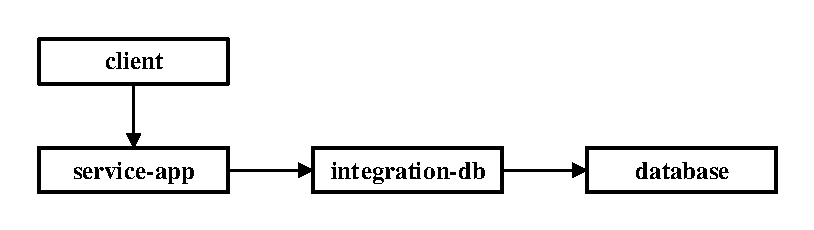
\includegraphics[scale=1]{images/esboc-design-services.pdf}
	\caption{Service Architecture}
	\label{fig:esboc-design-services}
\end{figure} 

\subsection{Client}
\label{sec:esboc-design-service-client}
The client will be a Java REST-Client which consumes data from the backing service application. The REST-Client could be a single page web application or an other back-end application. It will have no direct access to the database or the integration service, which integrates the database and the Service application, and is therefore completely abstracted of the underlying data storage and its schema.

\subsection{Service Application}
\label{sec:esboc-design-service-app}
The service application act as the back-end service for the client and produces data consumed by the client. The service application consumes from the integration service, which acts as the its back-end service. Same as the client, the service application is abstracted of the underlying data storage and its schema. 

\subsection{Integration Service}
\label{sec:esboc-design-service-integration}
The integration service acts as the front-end service of the database and the back-end service for the consumers. The integration service ensures that the consumers are abstracted of the underlying data storage and its schema, as well as that the database is accessed in a proper manner, by providing a public API which defines the operations and models.

\subsection{Database}
\label{sec:esboc-design-service-database}
The database acts as the data source for client which indirectly access this database via the integration service or a back-end service which itself is backed by the integration service. This level of abstraction of the consumers allows the database to evolve decoupled from the actual consumers. There is only the integration service which would have to be modified, when the underlying database or its schema changes.

\section{Service Requirements}
\label{sec:esboc-requirements-service}
In this section the service requirements will be specified, which will ensure that the services are properly implemented and can effortlessly be managed and monitored. Especially the management and monitoring becomes very important when moving from a conventional ESB application, like an application running on JBoss Fuse, to a microservice architecture, which is hosted on a PaaS platform like Openshift. Hosted on Openshift, the services run completely decoupled from each other with their own life cycle, which makes the management and monitoring harder compared to manage and monitor a monolithic application.

\subsection{Technology}
\label{sec:esboc-requirements-service-technology}
The services will be implemented in Java with the Java Enterprise Platform and the MicroProfile specifications. The MicroProfile specifications are an effort of the Eclipse Foundation to make Java applications ready for the cloud, where especially monitoring is a very important aspect to consider when it comes to distributed services. The services will be hosted as standalone applications like Spring Boot applications \cite{EclipseMicroprofileCharter2017, EclipseEE4JCharter2017}.

\subsection{State Handling}
\label{sec:esboc-requirements-service-state}
The service will be stateless, so that the services can be scaled and any request be handled by any instance of the service. Additionally Blue-Green-Releases and Canary-Releases are easily possible with stateless services \cite{FowlerBlueGreenRelease2010, FowlerCanaryRelease2010}. Multiple instances of stateful service hosted on a PaaS platform are not flexible as stateless services, because sessions must stick to a particular service instance, and persistence volumes have to be shared between the service instances.  

\subsection{Monitoring}
\label{sec:esboc-requirements-service-monitoring}
Monitoring is a essential aspect in distributed service architecture. Operators and developers need logging and tracing information of the services to comprehend errors in the services, where the cause of a problem could be located at another service as the service where a problem is reported.

\mysubsubsection{Distributed Tracing}
Distributed Tracing allows to comprehend service or method call chains. The MicroProfile specifications provides the OpenTracing specification, which provides an API for tracing an application on a method level or across service boundaries. The services must be able to collect tracing information about the REST and the related service method calls, and send this data to a central tracing service. The tracing implementation must be implemented separately from the service logic \cite{CNCFOpentracing2018}.

\mysubsubsection{Distributed Logging}
Distributed Logging allows to comprehend logs across service boundaries within a service call chain, where the logs of a service call chain have to be marked with a transaction id. The services must be able to provide all of their logging to a central service, whereby the logs are marked with a transaction id, which is equivalent to the transaction id of the service tracing. Optionally the services are allowed to add additional markers, which can help developers and operators to analyze problems or to group service logs.

\subsection{Configuration}
\label{sec:esboc-requirements-service-config}
The MicroProfile specifications provide the MicroProfile-Config specification, which provides an API to inject configuration parameters into classes, which can be loaded from different configuration sources. The services must provide the possibility to be configurable for different stages such as DEV (development), TEST (testing) and PROD (productive environment), where the services must not directly access the configuration sources, or hard code configuration in the source code unless its a default parameter \cite{EclipseMicroprofileConfig2018}.

\subsection{Fault Tolerance}
\label{sec:esboc-requirements-service-fault}
The MicroProfile specifications provide the specification MicroProfile-Fault-Tolerance, which provides an API to define fault tolerance behavior such as retries, timeouts and error fall-backs. The fault tolerance of a service means that, if a depending service is not accessible at the time, a service must not fail immediately after the first try, but the service should retry to call the depending service for several times, and fail when all retries have failed. Such a behavior ensures that short timed communication errors, redeployments or overloads do not immediately cause a service to fail. The services must provide proper fault tolerance configuration and fall-back behavior to be able to recover from such errors in a proper manner. \cite{EclipseMicroprofileFault2018}.   

\subsection{API Management}
\label{sec:esboc-requirements-service-api}
The API management of a public API such as REST-API REST-Models ensure that the clients, using a public API, are not broken by changes made on that API. There are several opinions on how API management can be done. Swagger has become very popular for documenting REST-API, where the documentation can be used to generate clients, provide documentation for developers and to test the public API. The services must be capable of migrating their public API in a way that the clients are not broken by the change. The replaced API version must be supported as well as the new one, so that the client is not forced to modify its source code \cite{SmartBearSwagger2018}.

\textbf{ADD resource which christoph found during liwestfsw research} 

\section{Openshift Architecture}
\label{sec:esboc-design-oc}

\subsection{Project}
\label{sec:esboc-design-oc-}

\subsection{Templates}
\label{sec:esboc-design-oc-config}

\subsection{Scripts}
\label{sec:esboc-design-oc-secrets}

\section{Openshift Requirements}
\label{sec:esboc-requirements-oc}

\subsection{Monitoring}
\label{sec:esboc-requirements-oc-monitoring}

\subsection{Configuration}
\label{sec:esboc-requirements-oc-config}

\subsection{Secrets}
\label{sec:esboc-requirements-oc-secrets}